%
% 3-tschebyscheff.tex
%
% (c) 2021 Prof Dr Andreas Müller
%
\section{Die Tschebyscheff-Polynome
\label{buch:polynome:section:tschebyscheff}}
Die Tschbeyscheff-Polynome sind ein Beispiel einer nützlichen Familie
von Polynomen, die wegen ihrer Anwendbarkeit durchaus den Rang von
speziellen Funktionen im weiteren Sinne verdienen.
Sie ermöglichen, Interpolationspolynome mit besonders guten
Fehlereigenschaften zu finden, haben aber auch andere Anwendungen
zum Beispiel beim Design von Filtern in der Elektronik.

%
% Motivation: Interpolation
%
\subsection{Motivation: Interpolation}
Nach dem Satz von Weierstrass
(Satz~\ref{buch:potenzen:satz:weierstrass})
lässt sich jede stetige Funktion auf einem kompakten Intervall durch
ein Polynom approximieren.
Interpolation kann zur Konstruktion solcher approximierender Polynome
verwendet werden, wie die folgenden Abschnitte zeigen sollen.
Die Optimierung des Approximationsfehlers führt auf die Spezifikation
einer interessanten Familie von Polynomen.

%
% Lagrange-Interpolationspolynom
%
\subsubsection{Lagrange-Interplationspolynom}
Eine mögliche Lösung des Problems, solche approximierenden Polynome
der Funktion $f(x)$
zu finden, besteht darin, ein Polynom $p(x)$ zu konstruieren, welches
in einzelnen, Stützstellen genannten Werten $x_0<x_1<\dots<x_n$ der
unabhängigen Variablen mit $f$ übereinstimmt, also
\[
p(x_i) = f(x_i), \quad i=0,\dots,n.
\]
Die Konstruktion eines solchen Polynoms geht aus vom Polynom
\[
l(x) = (x-x_0)(x-x_1)\cdots(x-x_n),
\]
welches an allen Stützstellen verschwindet.
Daraus lässt sich für jede Stützstelle ein Polynom
\[
l_j(x)
=
\frac{
(x-x_0)(x-x_1)\cdots\widehat{(x-x_j)}\cdots(x-x_n)
}{
(x_j-x_0)(x_j-x_1)\cdots\widehat{(x_j-x_j)}\cdots(x_j-x_n)
}
\]
konstruieren, wobei $\widehat{(x-x_j)}$ bedeutet, dass dieser Faktor
weggelassen werden soll.
Das Polynom $l_j(x)$ hat die Werte
\begin{align}
l_j(x_k)
&=
\frac{
(x_k-x_0)(x_k-x_1)\cdots\widehat{(x_k-x_j)}\cdots(x_k-x_n)
}{
(x_j-x_0)(x_j-x_1)\cdots\widehat{(x_j-x_j)}\cdots(x_j-x_n)
}
=
\delta_{jk}
=
\begin{cases}
1&\qquad j=k\\
0&\qquad j\ne k
\end{cases}
\label{buch:potenzen:interpolation:lj}
\end{align}
auf den Stützstellen.
Für $j\ne k$ enthält der Zähler von $l_j(x_k)$ den Faktor
$(x-x_k)$, der für $x=x_k$ verschwindet.
Daher verschwindet auch $l_j(x)$ für $x=x_k$.

\index{Lagrange-Interpolationspolynom}%
Das sogenannte {\em Lagrange-Interpolationspolynom} ist das Polynom
\[
p(x)
=
\sum_{j=0}^n f(x_j) l_j(x).
\]
Aus der Eigenschaft~\eqref{buch:potenzen:interpolation:lj} folgt, dass
\[
p(x_k)
=
\sum_{j=0}^n f(x_j) l_j(x_k)
=
\sum_{j=0}^n f(x_j) \delta_{jk}
=
f(x_k).
\]

%
% Fehler des Interpolationspolynoms
%
\subsubsection{Fehler des Interpolationspolynoms}
Der Approximationsfehler des Interpolationspolynoms kann mit der Formel
\[
f(x)-p(x)
=
l(x) \frac{f^{(n+1)}(\xi)}{(n+1)!}
\]
für einen geeigneten Wert $\xi$ mit $x_0 < \xi < x_n$.
Über die Ableitungen hat man natürlich keine Kontrolle, die einzige 
Möglichkeit, den Fehler möglichst klein zu halten ist daher,
die Sütztstellen so zu wählen, dass $l(x)$ kleine Funktionswerte hat.
Stützstellen in gleichen Abständen erweisen sich dafür als ungeeignet,
da $l(x)$ nahe $x_0$ und $x_n$ sehr stark oszilliert.

%
% Definition Tschbeyscheff-Polynome
%
\subsection{Definition der Tschebyscheff-Polynome
\label{sub:definiton_der_tschebyscheff-Polynome}}
\begin{figure}
\centering
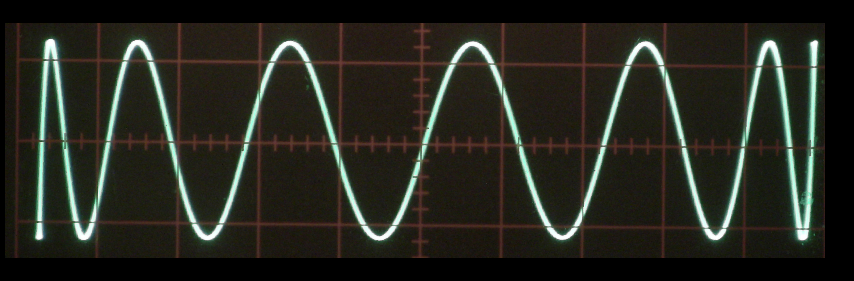
\includegraphics[width=\textwidth]{chapters/010-potenzen/images/lissajous.pdf}
\caption{Lissajous-Figur für zwei Signale $x=\cos t$ und $y=\cos 12t$.
\label{buch:potenzen:interpolation:lissajous}}
\end{figure}
\begin{figure}
\centering
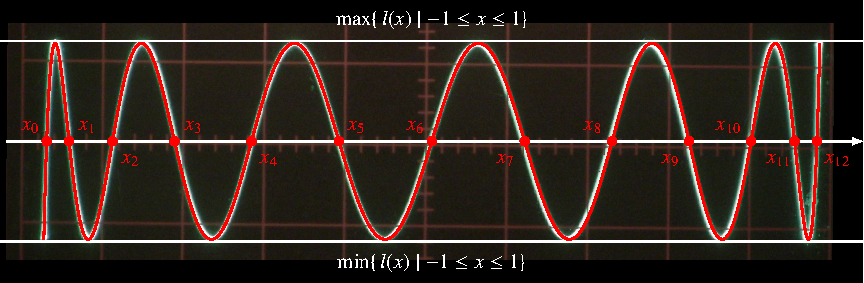
\includegraphics[width=\textwidth]{chapters/010-potenzen/images/lissajous-chebyshef.pdf}
\caption{Das Tschebyscheff-Polynom als Lösung des Interpolationsproblems.
\label{buch:potenzen:interpolation:lissajous-tschebyscheff}}
\end{figure}
Die Aufgabe, geeignete Stützstellen für das Interpolationsproblem zu finden,
die den Fehler minimieren, ist als gleichbedeutend damit, ein Polynom
zu finden, dessen Betrag beschränkt ist.
Eine Lissajous-Figur wie die in
Abbildung~\ref{buch:potenzen:interpolation:lissajous} erfüllt
diese Bedinung.
Sofern sie sich als Polynom ausdrücken lässt, könnte ihre Nullstellen
das Interpolationsproblem optimal lösen.

In der Lissajous-Figur in
Abbildung~\ref{buch:potenzen:interpolation:lissajous} ist
die Funktion $x=\cos t$ und $y=\cos 12t$ dargestellt.
Wegen $t=\arccos x$
Als Funktion von $x$ ist daher
\[
y(x) = \cos(nt)=\cos(n\arccos x).
\]
Tatsächlich ist aus der Theorie der trigonometrischen Funktionen
bekannt, dass die Kosinus eines Vielfachen des Winkels immer
als Polynom des Kosinus des Winkels dargestellt werden können.

\begin{definition}
\index{Tschebyscheff-Polynome}%
\label{buch:potenzen:def:tschebyscheff}
Das Polynom
\[
T_n(x)
=
\cos (n\arccos x),
\qquad
x\in[-1,1]
\]
heisst
{\em Tschebyscheff-Polynom (erster Art)} vom Grad $n$.
\end{definition}
Die Tschebyscheff-Polynome eignen sich auch hervorragend
dafür, Eigenschaften spezieller Funktionenfamilien zu
illustrieren.
Es wird sich zeigen, dass die Tschebyscheff-Polynome
Lösungen einer speziellen Differentialgleichung sind und
bezüglich eines in Kapitel~\ref{buch:chapter:orthogonalitaet}
definierten Skalarproduktes von Funktionen orthonormiert sind.

%
% Rekursionsbeziehungen
%
\subsection{Rekursionsbeziehungen
\label{buch:potenzen:tschebyscheff:rekursionsbeziehungen}}
Es ist etwas mühsam, einen Ausdruck von $T_n(x)$ direkt aus
trigonometrischen Identitäten herzuleiten.
In diesem Abschnitt soll daher eine Rekursionsbeziehung
hergeleitet werden.
Später in Abschnitt~\ref{buch:orthogonal:section:drei-term-rekursion}
wird gezeigt, dass solche Rekursionsbeziehungen eine Begleiterscheinung
orthogonaler Polynome sind.

%
% Drei-Term-Rekursion für die Tschebyscheff-Polynome
%
\subsubsection{Drei-Term-Rekursion für die Tschebyscheff-Polynome}
Mit der Abkürzung $y=\arccos(x)$ oder $x=\cos(y)$ bekommt man aus
der Definition~\label{buch:potenzen:def:tschebyscheff}
der Tschebyscheff-Polynome
\index{Drei-Term-Rekursion!für Tschebyscheff-Polynome}
\begin{align*}
xT_n(x)
&=
\cos(y)\cdot \cos(ny)
\\
&=
\frac12\bigl(
\cos((n+1)y) + \cos((n-1)y)
\bigr)
\\
x\,T_n(x)
&=
\frac12 T_{n+1}(x) + \frac12 T_{n-1}(x).
\end{align*}
Auflösen nach $T_{n+1}(x)$ ergibt
\begin{equation}
T_{n+1}(x) = 2x\,T_n(x)-T_{n-1}(x),
\quad
\text{mit Startwerten}
\quad T_1(x)=x,
\quad
T_0(x)=1.
\label{buch:potenzen:tschebyscheff:eqn:rekursion}
\end{equation}
Damit können die Tschebyscheff-Polynome sehr effizient berechnet werden:
\begin{equation}
\label{eq:tschebyscheff-polynome}
\begin{aligned}
T_0(x)
&=1
\\
T_1(x)
&=
x
\\
T_2(x)
&=
2x^2-1
\\
T_3(x)
&=
4x^3-3x
\\
T_4(x)
&=
8x^4-8x^2+1
\\
T_5(x)
&=
16x^5-20x^3+5x
\\
T_6(x)
&=
32x^6-48x^4+18x^2-1
\\
T_7(x)
&=
64x^7-112x^5+56x^3-7x
\\
T_8(x)
&=
128x^8-256x^6+160x^4-32x^2+1
\end{aligned}
\end{equation}
Die Rekursionsformel~\eqref{buch:potenzen:tschebyscheff:eqn:rekursion}
kann auch dazu verwendet werden, Werte der Tschebyscheff-Polynome
zu berechnen, wie in Übungsaufgabe~\ref{104} gezeigt wird.
Für $|x|>\frac12$ wird bei jeder Anwendung der Rekursion mit dem
Faktor $|2x|>1$ multipliziert.
Eventuell vorhandene Rundungsfehler werden natürlich ebenfalls
multipliziert und es besteht die Gefahr, dass diese exponentiell
schnell anwachsen.
Die Rechnung in Übungsaufgabe~\ref{104} zeigt aber, dass die
Resultate stabil auch für $n \approx 10^5$.

%
% Drei-Term-Rekursion für die Ableitung
%
\subsubsection{Drei-Term-Rekursion für die Ableitung}
Durch Ableitung der 
Rekursionsformel~\eqref{buch:potenzen:tschebyscheff:eqn:rekursion}
ist
\[
T_{n+1}'(x)
=
2T_{n}(x) + 2xT_n'(x) - T_{n-1}'(x).
\]
Die Anfangswerte sind $T_0'(x)=0$ und $T_1'(x)=1$.
Zusammen mit der
Rekursionsformel~\eqref{buch:potenzen:tschebyscheff:eqn:rekursion}
kann man also auch die Ableitungen effizient berechnen, zum Beispiel
für die Anwendung im Newton-Algorithmus.

%
% Multiplikationsformel
%
\subsubsection{Multiplikationsformel}
Aus der Definition mit Hilfe trigonometrischer Funktionen
lässt sich auch eine Multiplikationsformel ableiten.
\index{Multiplikationsformel}%

\begin{satz}
\index{Satz!Multiplikationsformel für Tsche\-by\-scheff-Po\-ly\-no\-me}%
Es gilt
\begin{align}
T_m(x)T_n(x)&=\frac12\bigl(T_{m+n}(x) + T_{m-n}(x)\bigr)
\label{buch:potenzen:tschebyscheff:mult1}
\\
T_{mn}(x) &= T_m(T_n(x)) = T_n(T_m(x))
\label{buch:potenzen:tschebyscheff:mult2}
\end{align}
für alle natürlichen $m$ und $n$.
\end{satz}

In \eqref{buch:potenzen:tschebyscheff:mult1} können negative Indizes
auftreten, wenn $n>m$ ist.
In solchen Fällen ist aber $T_{-n}(x)$ als
\[
T_{-n}(x)
=
\cos(-n\arccos(x))
=
\cos(n\arccos(x))
=
T_n(x),
\]
da die Kosinus-Funktion gerade ist.

\begin{proof}[Beweis]
Zunächst ist wieder mit der Abkürzung $t=\arccos x$
\begin{align*}
T_m(x)T_n(x)
&=
\cos mt \cos nt
=
\frac12\bigl(\cos((m+n)t)+\cos((m-n)t)\bigr)
=
\frac12\bigl(
T_{m+n}(x) + T_{m-n}(x)
\bigr),
\end{align*}
dies beweist~\eqref{buch:potenzen:tschebyscheff:mult1}.

Für \eqref{buch:potenzen:tschebyscheff:mult2} rechnet man
\[
T_m(T_n(x))
=
\underbrace{\cos(m\arccos(}_{\displaystyle T_m(}\underbrace{\cos(n\arccos x)}_{\displaystyle T_n(x)}\underbrace{))}_{\displaystyle)}
=
\cos(mn\arccos x)
=
T_{mn}(x).
\]
Damit ist auch \eqref{buch:potenzen:tschebyscheff:mult2} bewiesen.
\end{proof}

%
% Differentialgleichung
%
\subsubsection{Tschebyscheff-Differentialgleichung}
Die Ableitungen der Tschebyscheff-Polynome sind
\begin{align*}
T_n(x)
&=
\cos (ny(x))
&&
&&
\\
\frac{d}{dx} T_n(x)
&=
\frac{d}{dx} \cos(ny(x))
=
n\sin(ny(x)) \cdot \frac{dy}{dx}
&
&\text{mit}&
\frac{dy}{dx}
&=
-\frac{1}{\sqrt{1-x^2}}
\\
\frac{d^2}{dx^2} T_n(x)
&=
-n^2\cos(ny(x)) \biggl(\frac{dy}{dx}\biggr)^2 + n\sin(ny(x)) \frac{d^2y}{dx^2}
&
&\text{mit}&
\frac{d^2y}{dx^2}
&=
-\frac{x}{(1-x^2)^{\frac32}}.
\end{align*}
Wir suchen eine verschwindende Linearkombination dieser drei Terme
mit Funktionen von $x$ als Koeffizienten.
Wir setzen daher an
\begin{align*}
0
&=
\alpha(x) T_n''(x)
+
\beta(x) T_n'(x)
+
\gamma(x) T_n(x)
\\
&=
\biggl(
-\frac{n^2\alpha(x)}{1-x^2}
+
\gamma(x)
\biggr)
\cos(ny(x))
+
\biggl(
-\frac{nx\alpha(x)}{(1-x^2)^{\frac32}}
-\frac{n\beta(x)}{\sqrt{1-x^2}}
\biggr)
\sin(ny(x))
\end{align*}
Die grossen Klammern müssen verschwinden, was nur möglich ist, wenn zu
gegebenem $\alpha(x)$ die anderen beiden Koeffizienten
\begin{align*}
\beta(x)  &=  -\frac{x\alpha(x)}{1-x^2} \\
\gamma(x) &= n^2 \frac{\alpha(x)}{1-x^2}
\end{align*}
sind.
Die Koeffizienten werden besonders einfach, wenn man $\alpha(x)=1-x^2$ wählt.
Die Tschebyscheff-Polynome sind Lösungen der Differentialgleichung
\begin{equation}
(1-x^2) T_n''(x) -x T_n'(x) +n^2 T_n(x) = 0.
\label{buch:potenzen:tschebyscheff:dgl}
\end{equation}
Die Differentialgleichung~\eqref{buch:potenzen:tschebyscheff:dgl}
heisst {\em Tschebyscheff-Differentialgleichung}.
\index{Tschebyscheff-Differentialgleichung}%
\index{Differentialgleichung!Tschebyscheff-}%




